\section{Bayesian Belief Networks}
Suppose all features are \textbf{discrete} 
(if there are continuous and discrete, estimation is much more difficult)\\\\
Two key elements:\\
1. A directed acyclic graph (DAG) encoding dependence relationships between 
a set of variables\\\\
2. A probability table associating each node to immediate parent nodes

\subsection*{DAG: Conditional Independence}
A node in a Bayesian network is conditionally independent of its 
non-descendants, \textbf{if its parents are known}.
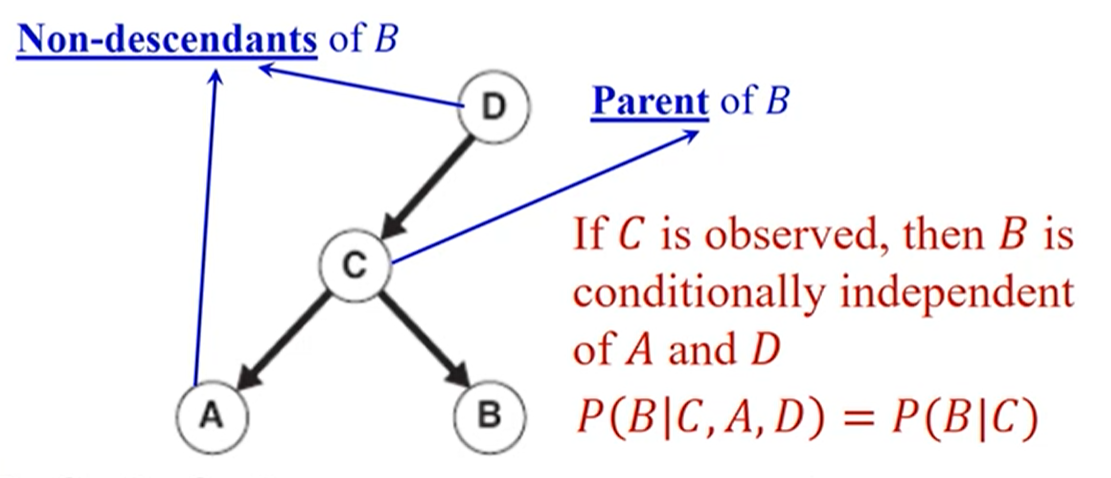
\includegraphics[width=\linewidth]{fig/bbn1}\\\\
\textbf{IMPORTANT!} If A and B are conditionally independent given C, we have:\\
1. $P(A|B,C) = P(A|C)$\\
2. $P(A,B|C) = P(A|C)P(B|C)$
\\

\subsection*{Important! Using BBN for Inference}
Given a BBN, and an inference(prediction) task:\\
1. Translate problem into probabilisitc language\\
2. If the probabilities to be estimated cannot be obtained 
from the probability tables of the BBN, then\\
A. Identify a subgraph which captures the dependence between 
input variables (features) and output variable (class)\\\\
B. Based on the network topology, apply product rule, sum rule
and the properties of conditional independence and independence
to induce equivalent forms of the probabilities until all 
probabilities can be found from the probability tables.